\documentclass[12pt]{article}
\usepackage{graphicx, float}
\usepackage[utf8]{inputenc}
\usepackage[T2A]{fontenc}
\usepackage[serbianc]{babel}
\usepackage {amsmath, amssymb, amsthm}
\graphicspath{{figures/}}

%   formatting
\usepackage[a4paper, top=1cm, bottom=1.5cm, left=2cm, right=1cm, heightrounded]{geometry}
\renewcommand{\baselinestretch}{1.15}
\setlength{\parindent}{0pt}
\setlength{\parskip}{0.8em}

\title{Дипломски Рад}
\author{Лазар Попадић}
\date{Август 2024}
%\maketitle

\begin{document}
\tableofcontents
\newpage

\section{Теорија}
\subsection{Машине једносмерне струје}
Машине једносмерне струје, у наставку МЈС, су електромеханички претварачи, који улазну електричну енергију претварају у механички рад. Састоје се из статора и ротора(арматуре). Статор успоставља побудно магнетно поље, због чега се назива и побуда. Кроз ротор се, преко четкица и комутатора, пропушта улазна арматурна струја. По принципу Лоренцовог закона $\vec F=Q(\vec v \times \vec B)$, индукује се сила која делује на ротор. Комутатор врши промену смера арматурне струје у зависности од положаја ротора, и тиме омогућава да Лоренцова сила увек делује у истом смеру, односно обезбеђује константан обртни момент мотора. Због Фарадејевог закона и Ленцовог правила $e_a=-N\dfrac{\partial\phi }{\partial t}$, обртање ротора индукује електромоторну силу супротног смера.

\begin{figure}[H]
    \centering
    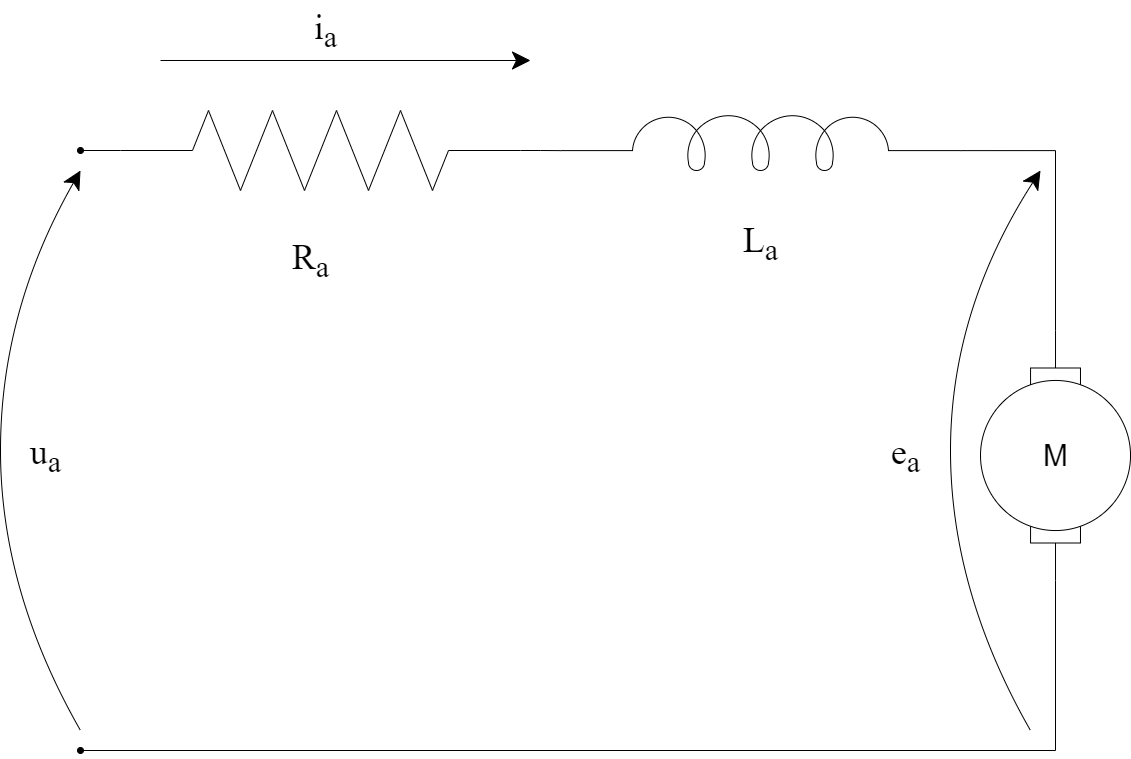
\includegraphics[width=12cm]{figures/ekv_kolo_armatura.png}
    \caption{Еквивалентно коло арматуре МЈС}
    \label{fig:коло_арматуре}
\end{figure}

\subsubsection{Динамички модел МЈС}
Модел МЈС се састоји из 2 подсистема: механичког и електричног, који међусобно интерагују. Посматраћемо МЈС која има сталну побуду јачинe магнетног флукса $\psi _f$. Модел се састоји из 3 диференцијалне једначине: напонске равнотеже арматурног навоја, механичке равнотеже и релације механичке брзине обртања и угла ротора. Као и из 2 алгебарске једначине: дефиниције електромагнетног момента и дефиниције индуковане електромоторне силе.
\begin{equation}
    u_a-e_a=R_ai_a+L_a\dfrac{di_a}{dt}
\end{equation}
\begin{equation}
    m_e-m_m=J_m \dot\omega+B_m\omega
\end{equation}
\begin{equation}
    \dfrac{d\theta}{dt}=\omega
\end{equation}
\begin{equation}
    m_e=\psi _fi_a
\end{equation}
\begin{equation}
    e_a=\psi _f\omega
\end{equation}
\newpage
Значења величина математичког модела МЈС:
\begin{itemize}
    \item $u_a$ - улазни арматурни напон
    \item $e_a$ - индукована електромоторна сила
    \item $R_a$ - електрична отпорност арматурног намотаја
    \item $i_a$ - арматурна струја
    \item $L_a$ - индуктивност арматурног намотаја
    \item $m_e$ - електромагнетни моменат
    \item $m_m$ - моменат оптерећења погона
    \item $J_m$ - моменат инерције обртних маса
    \item $\omega$ - угаона брзина арматуре
    \item $B_m$ - коефицијент пригушења брзине услед трења
    \item $\theta$ - угао ротора
    \item $\psi _f$ - јачина магнетног флукса побуде
\end{itemize}

\subsubsection{МЈС у стационарном стању}
Стационарно стање МЈС подразумева режим рада у којем су изводи променљивих стања по времену једнаки нули. Односно, арматурни напон и струја, моменат оптерећења и угаона брзина су константни. Овакво стање система је равнотежно и омогућава нам да лакше увидимо законитости утицаја улазних величина на излазне. Из једначина (2) и (4) следи:
\begin{equation}
    i_a=\dfrac{B_m\omega+m_m}{\psi _f}
\end{equation}
Уврштавањем (5) и (6) у (1):
\begin{equation}
    \omega(1+\dfrac{R_aB_m}{\psi _f^2})=\dfrac{u_a}{\psi _f}-\dfrac{R_am_m}{\psi _f^2}
\end{equation}
С обзиром да је коефицијент пригушења брзине $B_m$ типичног реда величине $10^{-6}$, можемо увести апроксимацију $B_m=0$. Тиме (6) и (7) постају:
\begin{equation}
    i_a=\dfrac{m_m}{\psi _f}
\end{equation}
\begin{equation}
    \omega=\dfrac{u_a}{\psi _f}-\dfrac{R_am_m}{\psi _f^2}
\end{equation}
Из (9) се може закључити да повећањем арматурног напона, угаона брзина линеарно расте, а повећањем момента оптерећења угаона брзина линеарно опада. Из тог закључка следи и идеја о регулацији брзине МЈС променом улазног арматурног напона.

\begin{figure}[H]
    \centering
    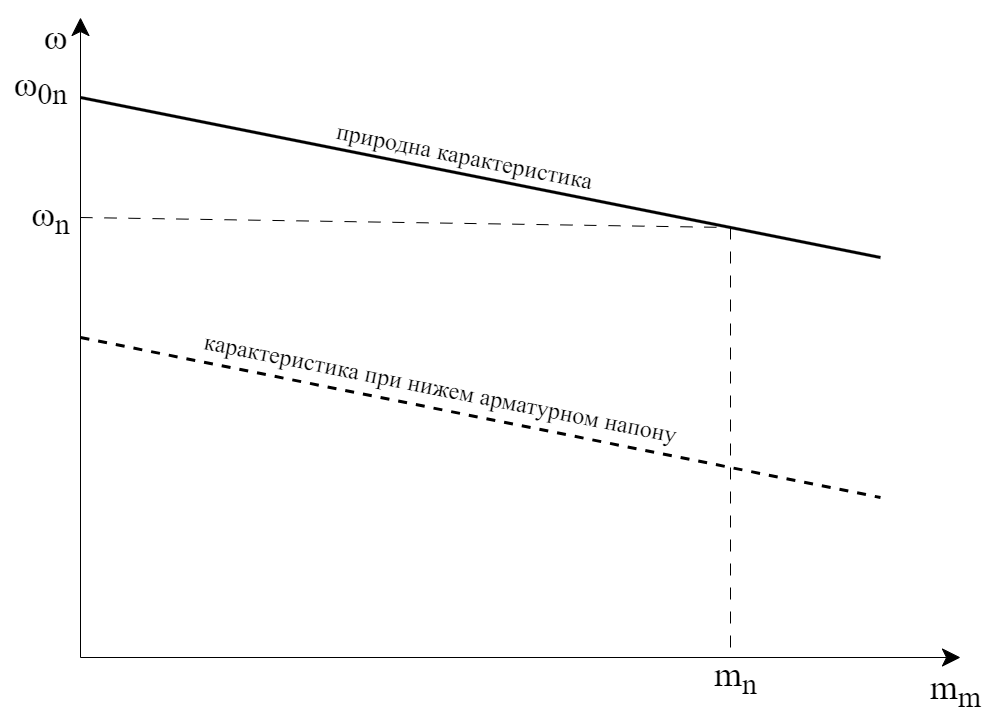
\includegraphics[width=15cm]{figures/k-ka_bdc.drawio.png}
    \caption{Механичка карактеристика МЈС}
    \label{fig:карактеристика_мјс}
\end{figure}

\subsection{PID регулација}
Регулација процеса представља управљање променљивама од значаја на основу управљачког алгоритма. Управљачки алгоритам представља функцију на основу које се генерише управљачки сигнал, на основу улазних сигнала. Основни захтеви регулације су: стабилност, тачност и брзина одзива. Два основна типа регулације су у затвореној и отвореној петљи. Односно, управљање са повратном спрегом и без повратне спреге. 

Регулација у отвореној петљи (open-loop control, non-feedback control loop) представља управљање у којем вредности излазних сигнала и сметњи немају утицај на управљачке сигнале. Овакви системи немају могућност отклањања грешака које су настале услед спољашњих поремећаја који делују на систем, или услед неидеалног познавања функционисања система. Системи који користе регулацију у отвореној петљи су спори системи који не захтевају велику прецизност и поновљивост.

\begin{figure}[H]
    \centering
    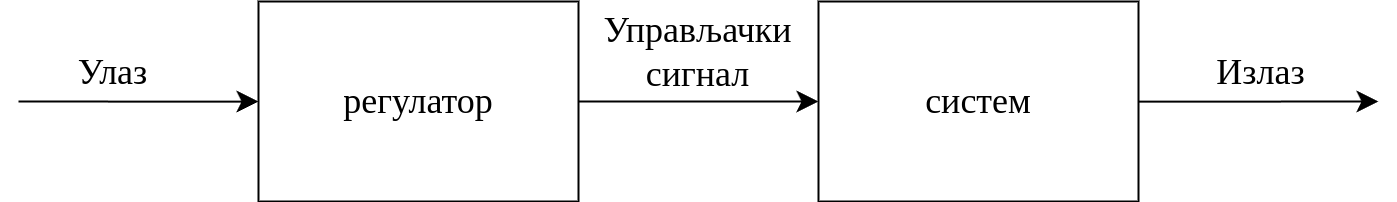
\includegraphics[width=14cm]{figures/open_loop.drawio.png}
    \caption{Блок шема управљања у отвореној спрези}
    \label{fig:отворена_спрега}
\end{figure}

Регулација у затвореној петљи (closed-loop control, feedback control loop) представља управљање у којем вредност управљачких сигнала зависи од разлике референтне(жељене) вредности и стварне вредности излазног сигнала. Овакви системи не захтевају идеално познавање управљаног система и имају могућност отклањања грешака услед спољашњих поремећаја.

\begin{figure}[H]
    \centering
    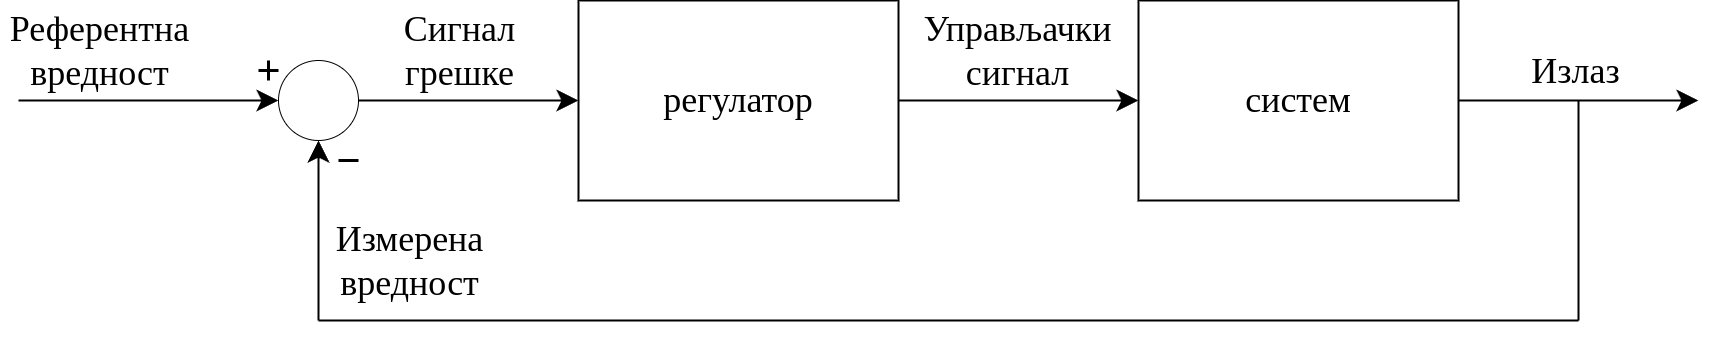
\includegraphics[width=15cm]{figures/closed_loop.drawio.png}
    \caption{Блок шема управљања у затвореној спрези}
    \label{fig:затворена_спрега}
\end{figure}

\subsubsection{Пропорцијално дејство}
Регулација на основу пропорцијалног дејства, односно P регулатори, представљају најједноставнији тип регулације са затвореном повратном спрегом. Управљачки сигнал представља сигнал грешке помножен фактором појачања пропорцијалног дејства:
\begin{equation}
    u_{(t)} = K_p e_{(t)},
\end{equation}
где $K_p$ предстаља фактор појачања пропорцијалног дејства, $u_{(t)}$ је управљачки сигнал, а $e_{(t)}$ је сигнал грешке. Сигнал грешке је једнак разлици референтне вредности и измерене вредности излаза, односно:
\begin{equation}
    e_{(t)}=y_{ref(t)} - y_{mer(t)}
\end{equation}
Функција преноса P регулатора у комплексном фреквенцијском домену је:
\begin{equation}
    G_{p(s)} = \dfrac{U_{(s)}}{E_{(s)}} = K_p
\end{equation}
\begin{figure}[H]
    \centering
    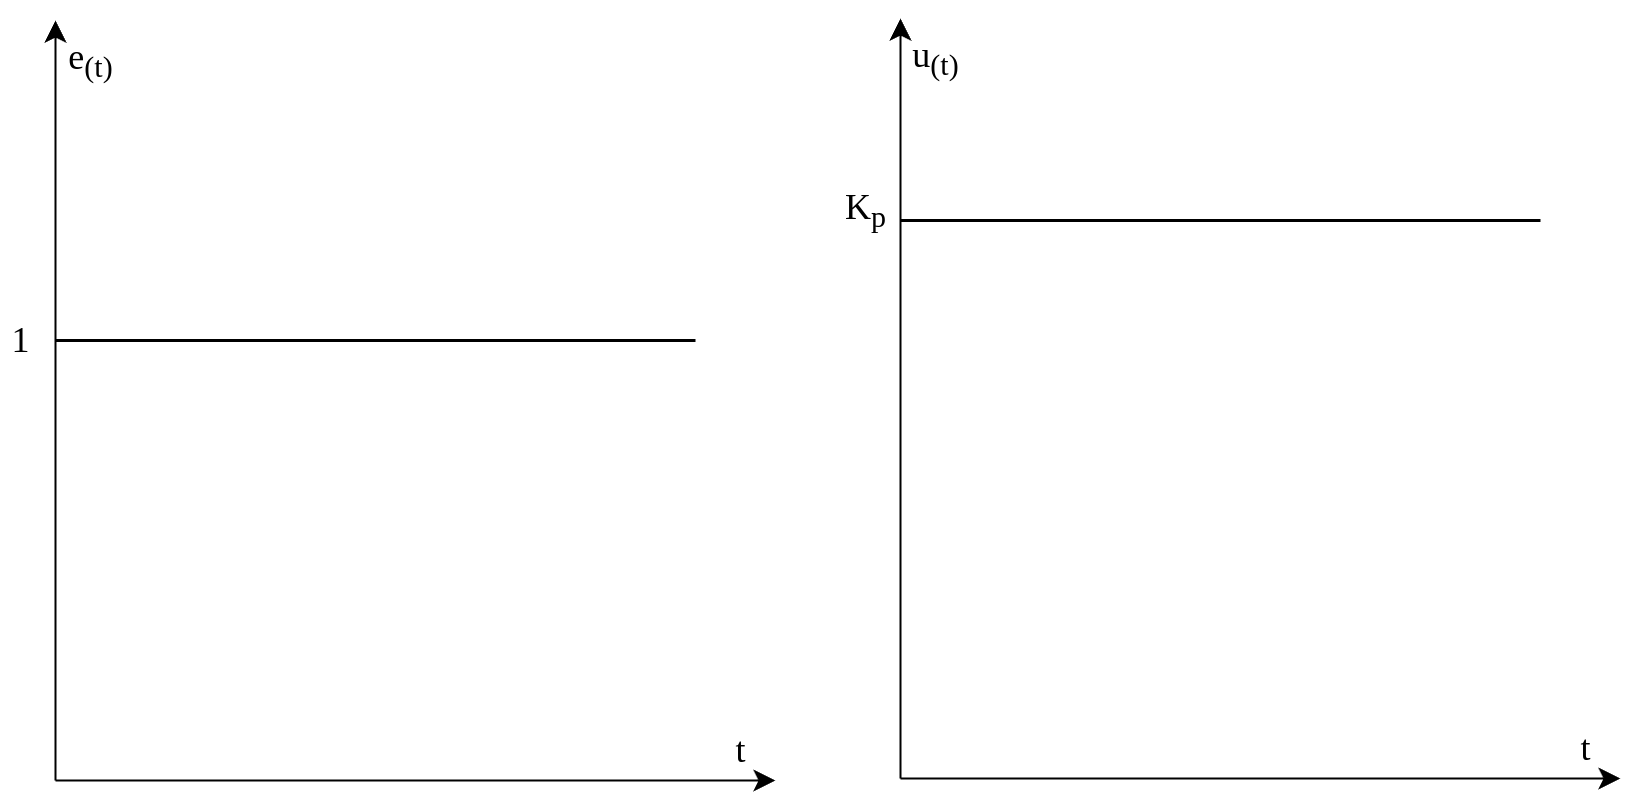
\includegraphics[width=13cm]{figures/p.drawio.png}
    \caption{Одзив P регулатора на одскочни сигнал грешке}
    \label{fig:P_одзив}
\end{figure}

\subsubsection{Интегрално дејство}
Регулација на основу интегралног дејства, односно I регулатори, су настали како би отклонили главну ману P регулатора. Та мана је могућност потпуног отклањања грешке у стационарном стању. I дејство негативно утиче на брзину одзива и на стабилност система. Управљачки сигнал I регулатора представља одређен интеграл сигнала грешке по времену, помножен фактором појачања интегралног дејства $K_i$:
\begin{equation}
    u_{(t)} = K_i\int_{0}^{t}e_{(t)}dt
\end{equation}
Функција преноса I регулатора у комплексном фреквенцијском домену је:
\begin{equation}
    G_{i(s)} = \dfrac{U_{(s)}}{E_{(s)}} = \dfrac{K_i}{s}
\end{equation}
\begin{figure}[H]
    \centering
    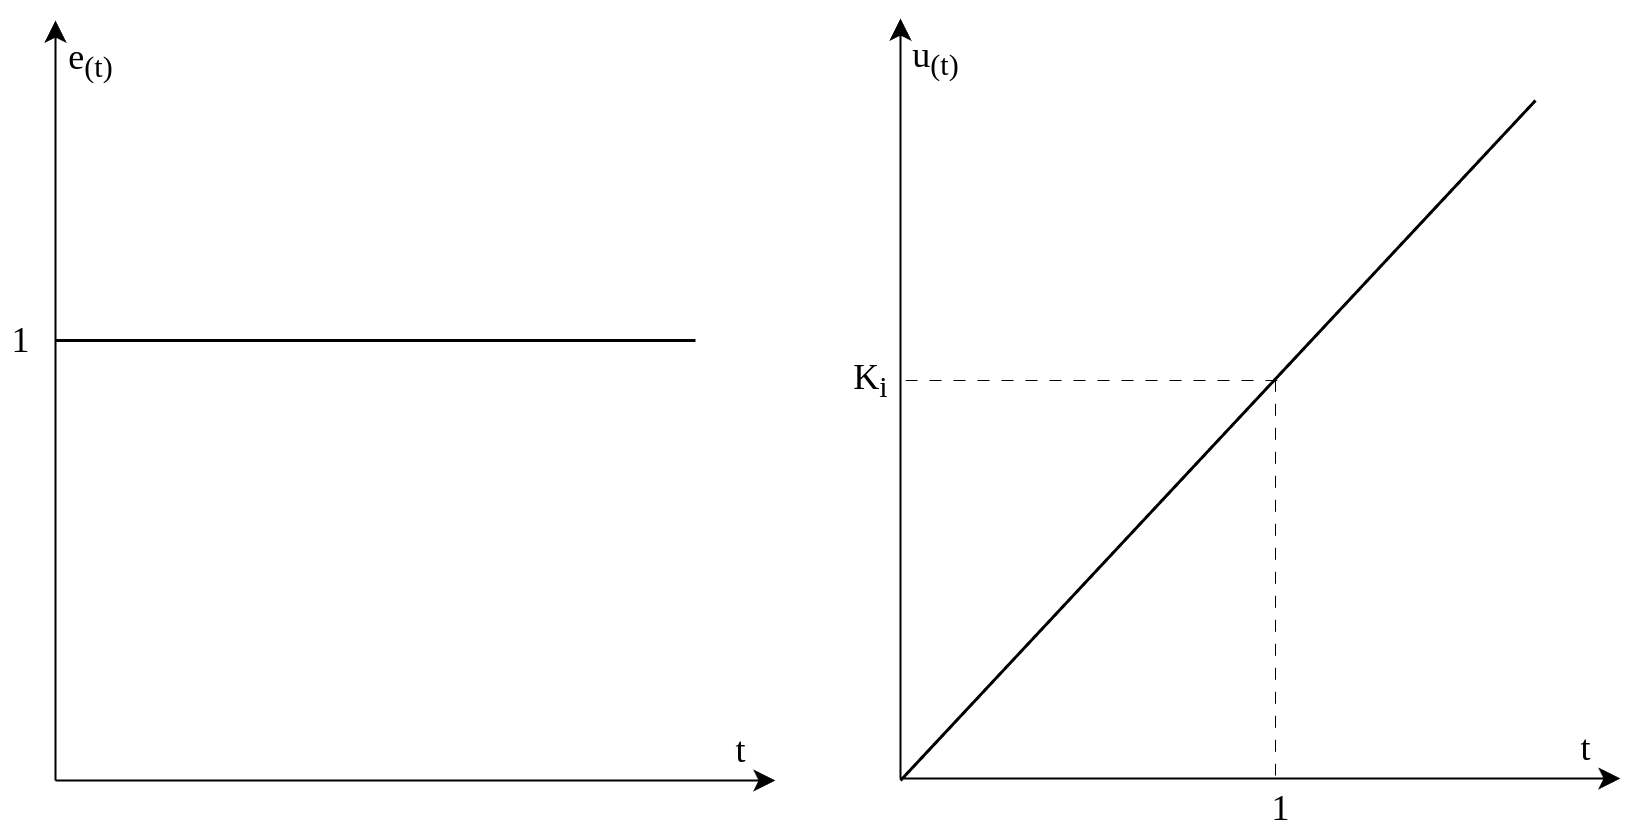
\includegraphics[width=13cm]{figures/i.drawio.png}
    \caption{Одзив I регулатора на одскочни сигнал грешке}
    \label{fig:I_одзив}
\end{figure}

\subsubsection{Диференцијално дејство}
Регулација на основу диференцијалног дејства, односно D регулатори, су настали како би отклонили мане I регулатора. Односно, како би убрзали одзив у прелазном режиму и смањили осцилације у устаљеном стању. Управљачки сигнал D регулатора представља извод сигнала грешке по времену, помножен фактором појачања диференцијалног дејства $K_d$:
\begin{equation}
    u_{(t)} = K_d\dfrac{de_{(t)}}{dt}
\end{equation}
Функција преноса D регулатора у комплексном фреквенцијском домену је:
\begin{equation}
    G_{d(s)} = \dfrac{U_{(s)}}{E_{(s)}} = K_ds
\end{equation}
\begin{figure}[H]
    \centering
    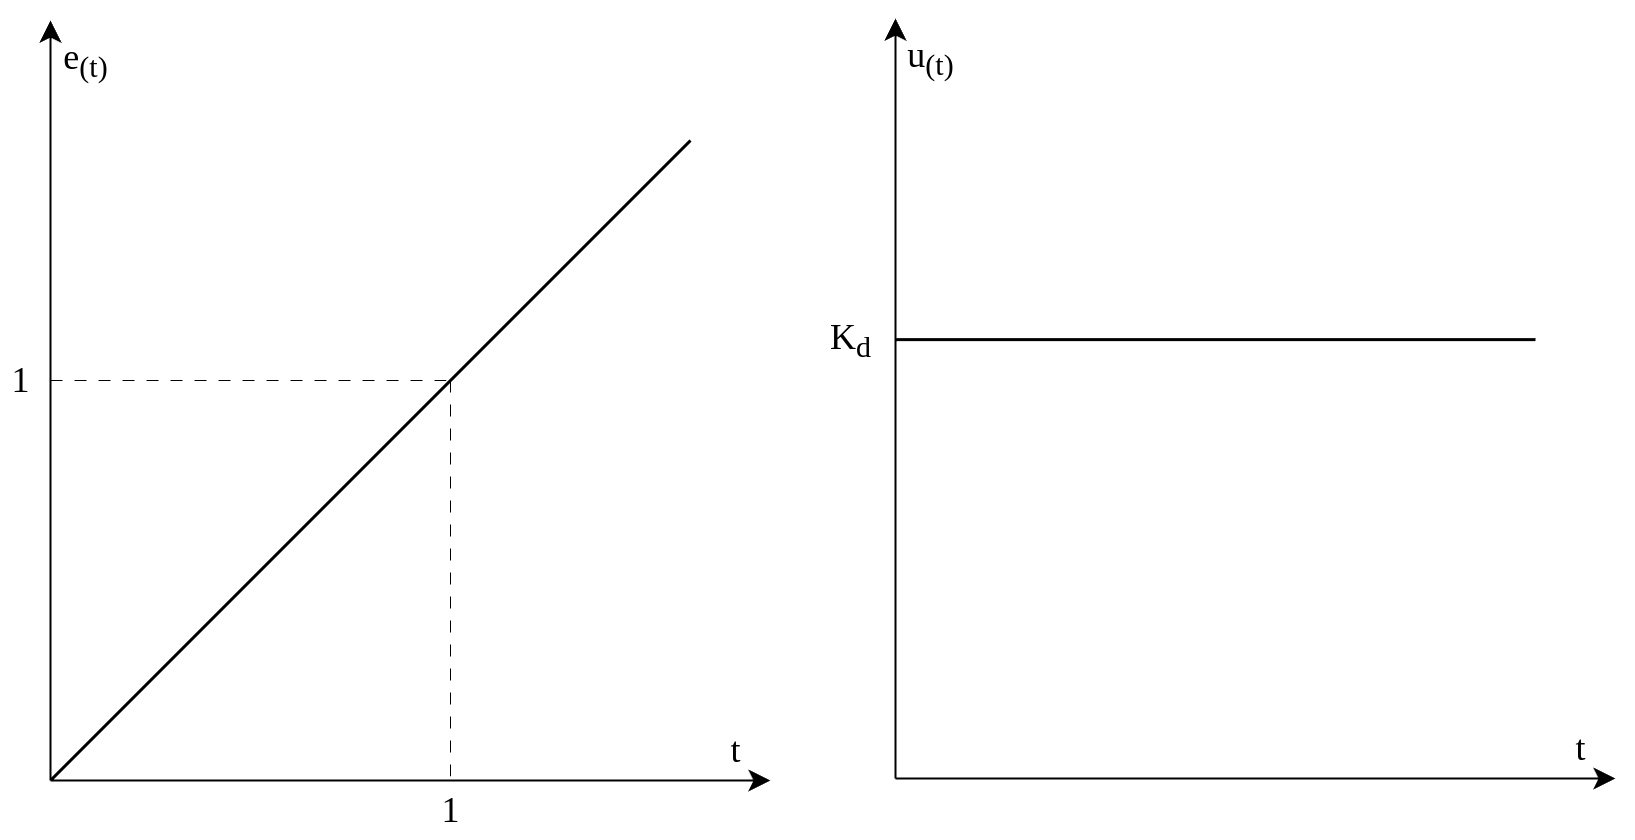
\includegraphics[width=13cm]{figures/d.drawio.png}
    \caption{Одзив D регулатора на сигнал грешке типа рампа}
    \label{fig:D_одзив}
\end{figure}

\subsubsection{PID}
PID регулатор настаје комбиновањем сва три претходно наведена дејства. Подешавањем фактора појачања пропорцијалног, диференцијалног и интегралног дејства могу се обезбедити жељене перформансе система.
Управљачки сигнал PID регулатора је:
\begin{equation}
    u_{(t)} = K_p e_{(t)} + K_i\int_{0}^{t}e_{(t)}dt + K_d\dfrac{de_{(t)}}{dt}
\end{equation}
Функција преноса PID регулатора у комплексном фреквенцијском домену је:
\begin{equation}
    G_{pid(s)} = \dfrac{U_{(s)}}{E_{(s)}} = K_p + \dfrac{K_i}{s} + K_ds
\end{equation}

\begin{figure}[H]
    \centering
    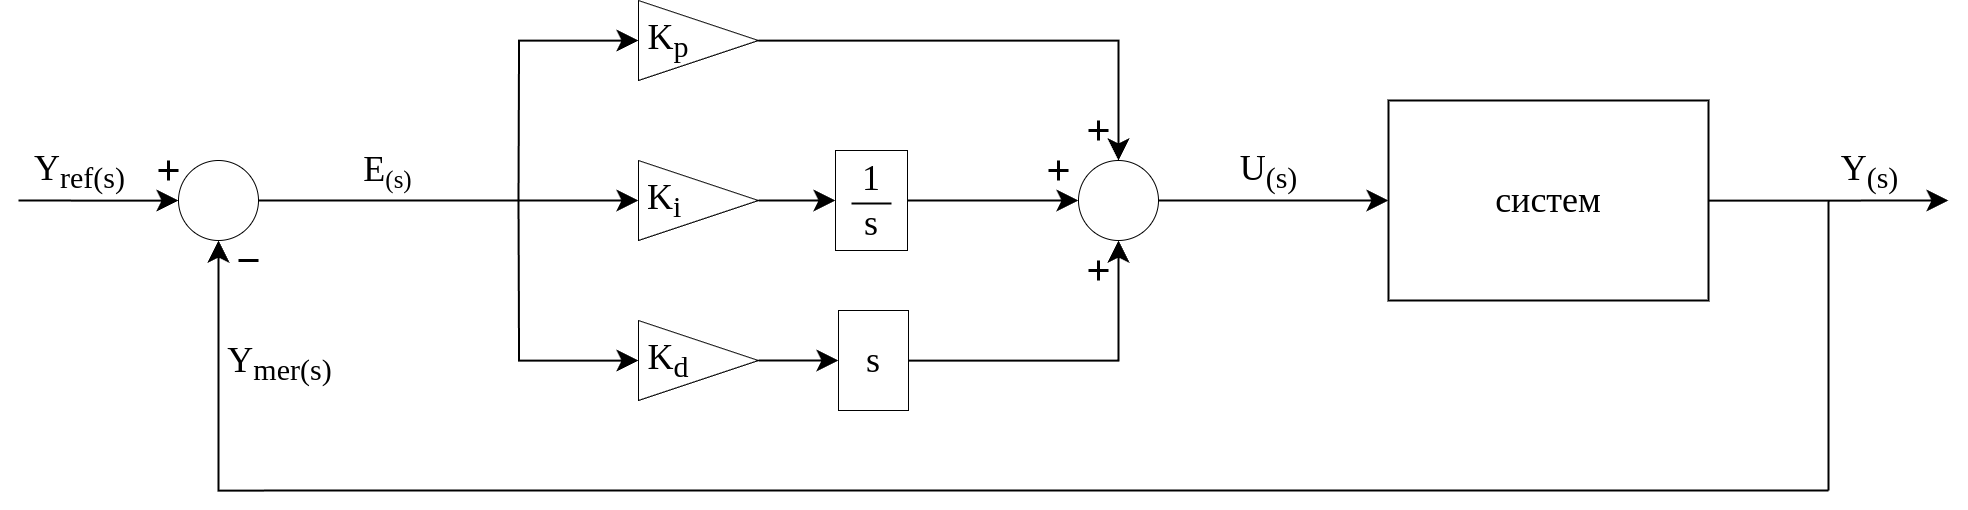
\includegraphics[width=18cm]{figures/pid.drawio.png}
    \caption{Блок шема PID регулатора у затвореној спрези}
    \label{fig:PID_затворена_спрега}
\end{figure}

\end{document}
